\documentclass[11pt]{report}
% packages
% Fran Burstall's Bath thesis package
\usepackage{baththesis}
\usepackage{amssymb} %for Blackboard bold etc \usepackage{graphicx} %for including eps graphics % front matter
\usepackage[pdftex]{graphicx}
\usepackage{url}

\title{ Illustrating how hydraulic machinery works } \author{Garoe Dorta-Perez}
%\degree{Doctor of Philosophy}
\degree{ Master of Science }
\department{Department of Computer Sciences} \degreemonthyear{January 2015}
\norestrictions

\begin{document}
\maketitle
\begin{abstract}
In this research proposal we present a method for automatic depiction of how it works illustrations of hydraulic machinery. \end{abstract}


\chapter{Introduction}
\label{ch:intro}

%1. Introduction to how things work visualization
\textit{How things work} visualizations have been used as an efficient method to explain how a wide range of systems work.
This technique usually involves displaying where each part is in relation to the system, showing how force is transmitted from one piece to the next and animating motion. 
In order to perform this task a range of visual transformations are used.
Such as viewing the system from different angles, zoom degrees,  transparency levels, as well as displaying only a subset of the parts.
Generating material of this sort typically involves manual methods, usually in the form of an expert drawing each illustration by hand or composing a fixed animation using specific software.\\

\begin{figure}
\centering
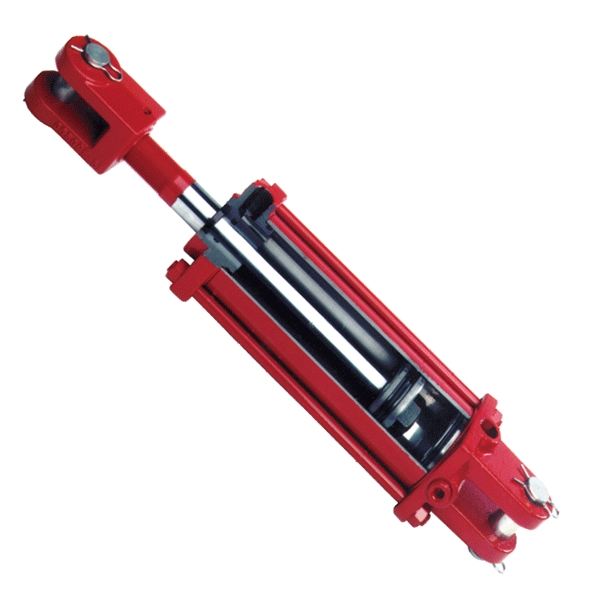
\includegraphics[scale=0.2]{images/h_pump}
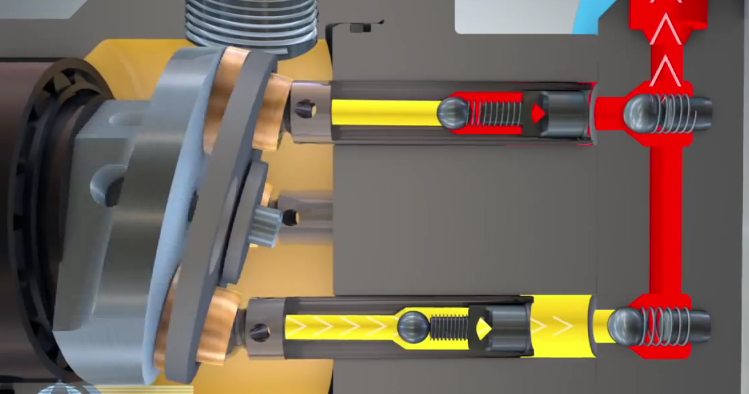
\includegraphics[scale=0.3]{images/cylinder_animation}
\caption{On the left a typical hydraulic cylinder cut in half, while on the right manually generated animation of a hydraulic pump.}
\label{fig:cylinder}
\end{figure}

%2. Introduction to hydraulics mechanisms
Hydraulic machinery is commonly used in our everyday lives.
Such as lifting cars with jacks, rams on excavators or gerotors to control fuel intake, as shown in Figure~\ref{fig:cylinder} left.
Their popularity is based on their faculty to transmit a force or torque multiplication independently of the distance between input and output.  
A typical hydraulic equipment has a contained liquid fluid that becomes pressurised when a force is applied to it.
Then that force is transmitted to the other end of the fluid. 
Understanding how the pressure is directed and how it interacts with other parts in the machinery is essential in order to grasp how the whole system works. 
Therefore, to illustrate the general process, the spatial configuration of each part in the system must be unveiled.
As well as the chain of motions that takes place within the gears and the liquid fluids.\\

%3. What are the visualization/illustration techniques for hydraulics mechanisms, refer to SIG10 gear paper.
There are some common visualisation and illustration techniques used for hydraulic machinery, as shown in Figure~\ref{fig:cylinder} right.
\textbf{Motion arrows} can point out how the solid parts move and they also indicate fluid flow movement.
\textbf{Frame sequences} display complex motions key frames and they can highlight temporal interactions between the parts.
\textbf{Animations} are an useful tool in highly dynamic systems, for example when an excessive number of frame sequences are needed in a particularly complex motion.\\

%4. Why this is difficult (designer need to understand force, flow movement, cannot change viewpoint, etc.)
Generating visualisations and illustrations for hydraulic machinery is challenging for designers.
They must understand in detail what forces are generated when the parts interact with each other and what kind of flow movements are entailed.
Furthermore, with 2D illustrations it is impossible to change the viewpoint to explore the object from different angle.
Moreover, hydraulic visualizations are usually costly animated by hand, which in addition leads to infrequent updates.\\

%5. Current status in the research field (mechanical assemblies SIG10, flow systems SIG ASIA 11, maybe some others? No need reference, just some general  discussion, since we have related work part also. And these work cannot handle hydraulics system)
There has been some work done on automatically generating illustrations and visualizations on mechanical assemblies.
Nevertheless, it has been restricted to gear to gear interaction only.
Whereas work on fluid simulation and visualization has not been applied to hydraulic equipment.
As they are usually designed to, either generate complex visualizations for engineering purposes, or at producing visually plausible but not physically accurate results in animation and games.\\

%6. Our aim (analysis + visualization, with some description, refer to SIG10 gear paper)
Simulations can be used to illustrate how hydraulic machinery works.
This research proposal aims to introduce a method for generating \textit{How things work} illustrations for hydraulic machinery.
This illustrations would help users understanding how this kind of equipment works.\\

%7. Summarize our contribution
In summary, the main contributions would be:
\begin{itemize}
\item An application for creating how things works illustration for hydraulic machinery 3D models.
\item A method for detecting motion and interaction of fluid inside model parts.
\item Algorithms to automatically generate illustrations with motion arrows and frame sequences
\end{itemize}

%Reference example
% Chapter \ref{ch:intro}

\section{The Problem}
\label{sec:problem}

Given a 3D CAD model of some hydraulic machinery we want to generate how things work visualizations.
Namely, adding arrows depicting the fluid movement.\\

The problem can be subdivided into:
\begin{enumerate}
\item Part analysis: Detecting fluid containers and fluid handling parts.
\item Fluid simulation: Simulate how the fluid behaves in the previously detected parts.
\item Fluid visualization: Display the fluid simulation data in a intuitive format.\\
\end{enumerate}

Part analysis involves detecting the part type, how it moves and interacts with others.
So the information saved for type would be gear, cylinder, valve, reservoir, etc.
In this section there is a clear difference between the parts that interact with fluids and the ones that do not. 
With respect to types of movement, it would be direction of movement, axis of rotation, axis of translation, etc.\\

Once the parts have been categorized and given an input force, we will have to simulate how the force is transmitted along the different parts.
In the special case where a part is a container of a fluid or is in direct contact with one, that force will have to be introduced in a fluid simulation algorithm.
The output of the simulation will then carry the information along to the next parts.\\

Lastly, in order to visualize the fluid simulation data we will need to generate a visual cue that will indicate intuitively the fluid movement.
A simple approach would be to place arrows indicating the overall fluid movement.

\section{Previous Work}

This proposal is based on the following three main areas of previous work.

\subsection{Explanatory illustration}

Explanatory illustration has been effectively used to show either complex and/or copious amounts of  scientific, as well as simple dynamics as the ones found in comics books.
Nienhaus proposed a technique to depict motion in 3D animations~\cite{Nienhaus2005}.
Scene and behaviour descriptions from specialized scene graphs were analysed in order to create the motion cues.  
Researchers have have look into generate automatic illustrations for mechanical assemblies \cite{Mitra2010}.
Furthermore, Lowe showed that even though animations have become a generalized tool for visualizing dynamic systems, special care have to be taken as users can fail at extract the necessary information due tu the nature of the animation~\cite{Lowe2014}.
%TODO Improve and extend this, but it is difficult to find literature on this topic


\subsection{Fluid simulation}

Fluid simulation is a well known research area. 
One of the firsts papers in this area introduced a Grid method \cite{Foster1996} to solve Navier-Stokes equations by applying forward Euler time integration. 
Stam \cite{Stam1999} extended this method in order to overcome stability issues.
More recent simulations introduced the Smooth Particle Hydrodynamics (SPH) technique \cite{DesbrunMathieuandGascuel1996}.
However the previous techniques assumed the fluid to have no interplay with any rigid body (solid-coupling).
Carlson \cite{Carlson2004} proposed solid-fluid coupling algorithm for grids models using distributed Lagrange multipliers.
On the other hand, Muller \cite{Muller2004} presented his own method for SPH simulations, which Akinci \cite{Akinci2012} further improveded with the inclusion of friction and dragging. 
Shao \cite{Shao2014} also solved stability issues in the previous SPH solid-fluid coupling techniques.
For more information on real time fluid simulations see Vines survey ~\cite{Vines2012}.
While for survey specific to SPH fluid simulation see Ihmsen~\cite{Ihmsen2014}.

\subsection{Flow visualization}

%Explain what stream lines are, why thy are used and some applications on flow visualization
Extensive work has been done in this area as visualizing fluid movement has a broad range of applications. 
Streamlines are a common tool to visualize flow.
A streamline is defined as curve that is everywhere tangent to flow field.
Therefore, they provide an intuitive show the direction the fluid will travel.
%Define this better, explain more nice properties of the stream lines
Furthermore, their curvature is related to the pressure gradient.\\

On the 2D image domain, an image-guided algorithm for visualizing 2D flow in images was proposed by Turk \cite{Turk1996} and which Li improved to use the fewest number of streamlines \cite{Li2008}. \\

Seeding techniques for curves on 3D surfaces were explored by Wicke \cite{Wicke2009}, who developed a technique to combine model reduction with with grid based methods.
And Spencer \cite{Spencer2009} whose method generates streamlines only for visible parts of the surface, thus providing a significant gain in efficiency.
For more information on flow visualization see McLoughlin survey on the topic~\cite{McLoughlin2010}.

%Sould this section go before the previous work or where it is now????
\section{Related Work}

%Talk here about Illustrating how mechanical assemblies work
%sketch based dynamic illustration of fluid systems

\chapter{Data Structures Used in this research}
\section{The 4D-Stack - A Revolutionary Data Structure}
The 4D-Stack turned out to be a complete disaster as traversal time approached $O(n^9).$
It is best illustrated by the following equation: $F(x) = \prod_{0\leq i<k}d_i(x)$
but the following may not be true:

\[
-f(x) = - \log \prod_{0\leq i<k}d_i(x) = - \sum_{0\leq i<k} \log d_i(x)
\]


\section{More Irrelevant Stuff}
If you want to put numbers on equations use this form:
\begin{equation}
\label{integralrep}
f(x)=\int_0^L h( \langle x-p(t),n(t) \rangle ) dt\,.
\end{equation}



\chapter{Results}

Due to a time quake during the research, the results were catapulted into the future.  They will appear in about 20 years.
In the meantime to demonstrate the use of tables, please see table~\ref{stud-table} for a list of students who took more than 30 years to graduate.

\chapter{Conclusions and Future Work}
No conclusions can be drawn until the results appear and no future work is recommended.

\bibliographystyle{eg-alpha-doi}

\bibliography{baththesis}


\end{document}
